\newpage
\section{Monetary Transmission Channels} \label{sec:MonetaryTransmissionChannels}
In his paper \footcite[See.][]{Mishkin1996}, Mishkin gives an overview of the transmission mechanisms of monetary policy in economy. Most important channels are namely interest rate channel, asset prices and credit channel. In the following sections we review this paper and explain every channel in detail. 

\subsection{Interest Rate}
Interest rate channel is explained with the traditional Keynesian \ac{ISLM} and shows the effects of a monetary expansion as follows:
  \[M \uparrow \implies r \downarrow \implies I \uparrow \implies Y \uparrow\]
where $ M \uparrow $ indicates expansionary monetary policy which leads to fall in real interest rate $r$, which lowers the cost of capital, causing rise in investment spending $I$, therefore resulting in an increase in output $Y$.

\subsection{Asset Price Channels}
According to Mishkin \footcite[See.][]{Mishkin1996} the exchange rate channel can be illustrated as follows:
 \[M \uparrow \implies r \downarrow \implies E \downarrow \implies NX \uparrow\ \implies Y \uparrow\]
An expansionary monetary policy leads to fall in domestic real interest rate. As a consequence, domestic currency$E$  becomes less attractive in comparison to other currencies. Depreciated currency makes domestic good more attractive for export. As a result net export $NX$ raises followed by aggregate output. 
Furthermore,  two sub-channels are introduced for equity price namely Tobin's q and Wealth Effects \footcite[See.][]{Mishkin1996}. 
Tobin's q can be summarized as following \footcite[See.][]{Mishkin1996}: 
 \[M \uparrow \implies P_e \uparrow \implies q \uparrow \implies I \uparrow \implies Y \uparrow\]
Higher equity prices $P_e$ leads to a higher $q$ factor (market value of the firm divided by replacement cost of capital). When $q$ is high companies issue equities and buy new investment goods which are relatively cheaper so investment increases. 
The wealth channel is described as follows \footcite[See.][]{Mishkin1996}: 
\[M \uparrow \implies P_e \uparrow \implies wealth \uparrow \implies consumption \uparrow \implies Y \uparrow\]
Housing and land price which is our topic of interest in this work can be categorized in this channel as equity.

\subsection{Credit Channels}
Two basic channels of monetary transmission emerged because of asymmetric information are Bank Lending and Balance Sheet channels. 
Bank Lending Channel \footcite[See.][]{Mishkin1996}:
This transmission channel is very straightforward:
 \[M \uparrow \implies bank deposits \uparrow \implies bank loans \uparrow \implies I \uparrow\ \implies Y \uparrow\]
Increased bank reserves and available loans causes investment to rise.
Balance Sheet Channel \footcite[See.][]{Mishkin1996}:
 \[M \uparrow \implies P_e \uparrow \implies adverse selection and moral hazard \downarrow \implies lending \uparrow \implies I \uparrow \implies Y \uparrow\]
Expansionary monetary policy raises the cashflow and consequently reduces adverse selection and moral hazard (risk) and therefore more lending.

\subsection{Housing Related Transmission Channels}

Among all the channels explained in previous sections, a very concise representation of the housing market related channels are shown in Figure \ref{fig:HousingTransmission}
\begin{figure}[H]
\caption{Monetary Transmission Channels Affecting the Housing Market }\label{fig:HousingTransmission}
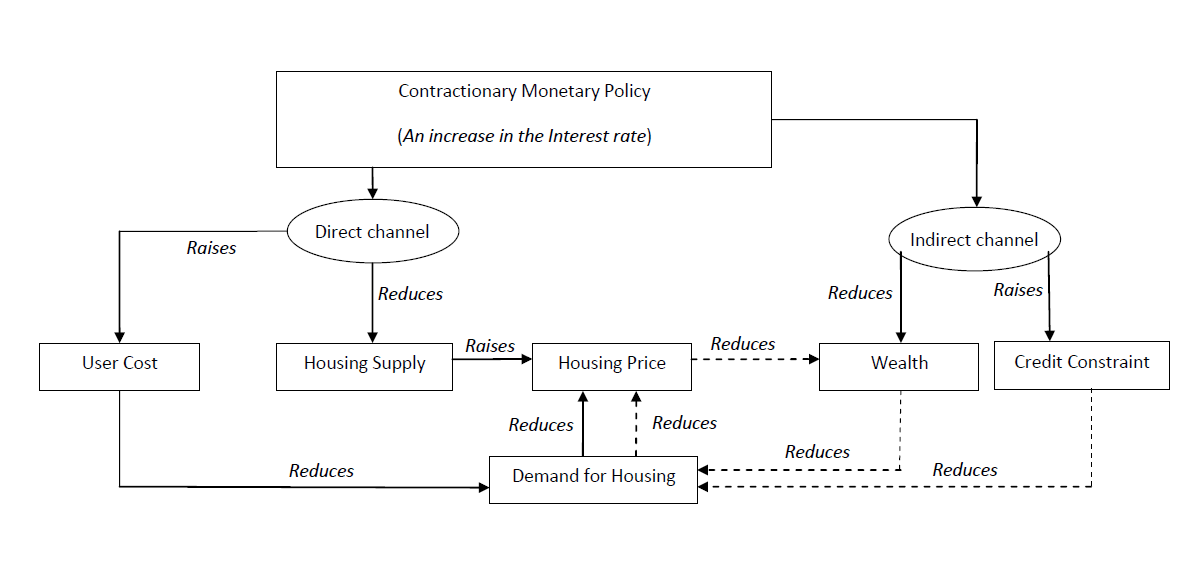
\includegraphics[width=0.9\textwidth]{HousingTransmission}
\\
\cite[Source: See][]{Wadud2009}
\end{figure}

Following his older paper on monetary transmission channels, Mishkin concentrates merely on housing market in his more recent paper~\footcite[See.][]{Mishkin1996} and explains these channels as follows:
\subsubsection{Direct Channels}
Direct Interest Rate Effects through the User Cost of Capital

The user cost of housing capital can be described as ~\footcite[See.][]{Mishkin2007}
 \[ uc = hp((1-t)i - \pi_e) - (\pi_h - \pi_e) + \delta \]
 whre $uc$ is user cost of capital, $hp$ is the relative purchase price of new housing capital, $i$ is the mortgage rate and $\pi_h$ and $\pi_e$ are the appreciation of housing prices and real inflation. $\delta$ is depreciation rate for housing. The formula also deductible mortgage interest by adjusting the nominal mortgage rate by the marginal tax rate $t$ after tax real interest rate. One can see that when the interest rate raises the user cost of capital raises  and consequently the demand for housing decreases. The fall in demand result in a fall in supply and consequently aggregate demand. Looking more precisely in $(\pi_h - \pi_e)$ part of user cost equation one can see the effect of interest rate. When interest rate raises the expected appreciation of housing price falls and therefore the current user cost of capital increases which in turn result in decline in demand. 

Interest Rate Effect on Supply \footcite[See.][]{Mishkin2007}
Higher short-term rates, which increase cost of supply and decreases housing activity.

\subsubsection{Indirect Channels}
There exist evidences proving an increase in wealth should have positive effect on consumption\footcite[See.][]{Mishkin2007}. As we know from previous section an expansionary monetary policy can increase the demand for housing which normally leads to in increase in house price. Therefore, total wealth and consequently aggregate demand increases.
Moreover, an increase in house price improves the house hold balance sheet and reduces the risk for the credit giver as explained in previous sections.

\subsection{Data Analysis}\label{sec:Data}
In this section we introduce the variables which in our opinion play a role in housing sector of economy. The data evidence from German market and the sources of data are introduced. 
\subsubsection{Interest Rate} 
\ac{r} is the money market interest rate \footcite[See.][]{BundesBank} (EONIA). It is the rate at which banks provide loans to each other with a duration of 1 day, In my opinion this is a good indicator of the monetary policy since it combines central banks ECB's deposit facility rate and ECB interest rates for main refinancing operations. This affect is more clear when we look in the recent data after 2018 where central banks interest rate for refinancing is zero but the deposit facility goes negative and this stimulates banks to lend more money. Original data is monthly and we need to average to get the yearly rate. 

\subsubsection{Government Spending} 
General government deficit(-) or surplus(+) as defined in the Maastricht Treaty \footcite[See.][]{BundesBank} is used to describe \ac{rg}. In my opinion, it is a good indicator of the Government fiscal policy since it includes both expenditure and earning of the government. Change in percentage for each year is calculated and sign is reversed such that when the government has a deficit it is an indicator if positive government spending.

\subsubsection{Output} 

\ac{ry} is represented by the data from German overall econonmy \footcite[See.][]{BundesBank}.

\subsubsection{Material Cost} 

\ac{mc} is represented by the construction price index \footcite[See.][]{BundesBank}.

\subsubsection{Housing Price} 
\ac{hp} is represented by the data from OECD \footcite[See.][]{OECD}.

\subsubsection{Housing Supply} 
For \ac{h}, west Germany's data from Statista\footcite[See.][]{Statista} is used. Although this data is only for west Germany, we assume that it represents the trend in the whole country.

\subsubsection{Data Analysis} \label{subsec:dataAnalysis}
If we look into Figure \ref{irhp} and take the period 2008 till 2011 as an example into account, we can see that an expansionary monetary policy  (increase in \ac{r}) together with an increase in government spending (raise in \ac{rg})  have resulted in appreciation of the housing price. This change in the house price is expected as we described in chapter \ref{sec:MonetaryTransmissionChannels}.   

\begin{figure}[H]
\caption{Interest Rate, Government Spending and House Price in Germany in Years 2000-2020}\label{irhp}
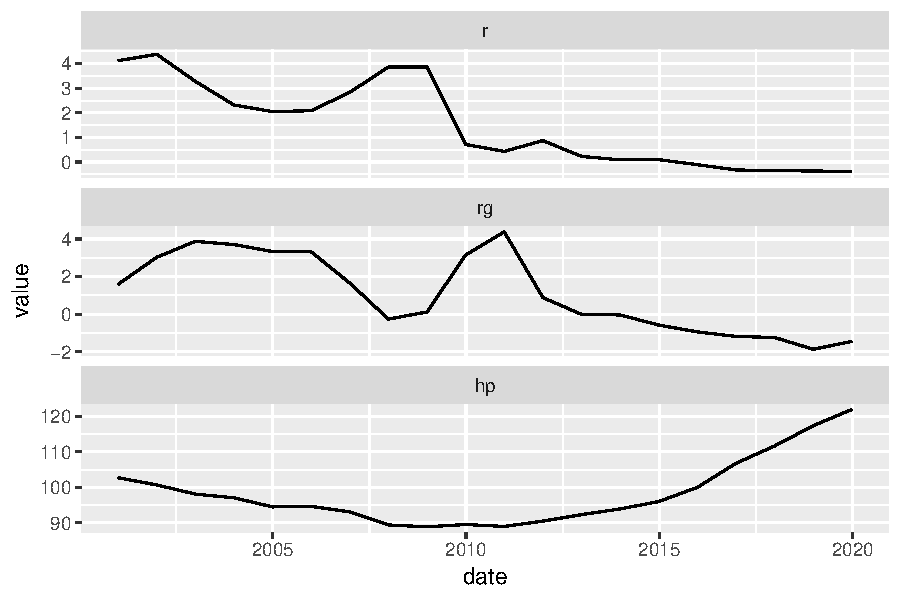
\includegraphics[width=0.9\textwidth]{interesetRateOnHousePrice}
\\
Source: Own Figure
\end{figure}

Moreover, if we look into Figure \ref{irgdp} and take the period 2008 till 2011 as an example into account, we can see that an expansionary monetary policy had led to an increase in housing supply and consequently the aggregate output of the economy. This relationship is expected as we described previously in \ref{sec:MonetaryTransmissionChannels}.   



\begin{figure}[H]
\caption{Interest Rate, Housing Supply and GDP in Germany in Years 2000-2020}\label{irgdp}
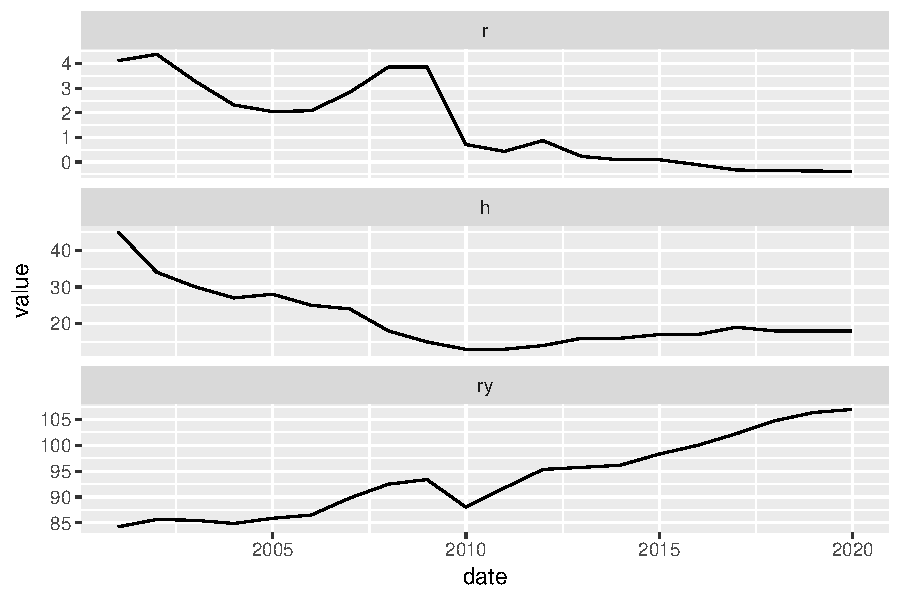
\includegraphics[width=0.9\textwidth]{interestRateOnOutput}
\\
Source: Own Figure
\end{figure}






